\documentclass[]{article}

\usepackage{amsmath}
\usepackage{graphicx,color,psfrag}

\usepackage{epstopdf}

\usepackage{hyperref}
\usepackage{cleveref}
%opening
\title{Statistical Methods in Fast Fracture of Ceramics}
\author{Burak ER}

\begin{document}

\maketitle

\begin{abstract}
Ceramic materials are brittle and their fracture shows probabilistic behavior which makes it impossible to use classical fracture theory. Statistical fracture methods are developed to overcome this problem and they are very handy and the only tool that are available. They are all based on Weibull's theory. In this article, the theory background of the statistical methods of fast fracture of ceramics is first given then the required experimental procedures is mentioned. A computer code CARES that is probably the only publicly available numerical source for the computer based statistical analysis is also presented.
\end{abstract}

\section{Introduction}
Ceramic materials are very important for many kind of engineering branches and have many kind of different 
use cases. In most of the applications they stand on the core of these applications, thus, their role is to make possible of the main 
functionalities. For example; ceramics give hardness to the cutting tools, 
refractivity and low friction to the internal combustion engine blocks. Therefore, their failure results completely unusable machines. 

Fracture is an important type of failure of the ceramic materials. As a result of variable severity of inherent flaws in ceramics, 
they are highly brittle and unlike metals, they exhibit large variation on their fracture toughness from specimen to specimen. Therefore, 
the strength of ceramics show probabilistic behavior thus prediction of the failure of ceramic materials is hard. 
This nature makes use of statistical methods is a must for the fracture predictability of ceramic materials.

\section{Statistical Methods}  
\subsection*{Weibull's Method}
First statistical treatment of the prediction of fracture of ceramic materials was that of Weibull's\cite{weibull1939}. Weibull exploited the analogy between a stressed brittle structure and a loaded chain, which breaks when the strength of its weakest link is exceeded. All current methods are based on his ideas, thus, the so called Weakest Link Theory(WLT).

Weibull started the development of his ideas with considering a rod that is under tensile stress, then, defined the term risk of rupture for a volume element as
\begin{align}
d B &= -\ln{\left(I-S_0\left(\sigma\right)\right)}d V
\end{align}
and probability of failure as
\begin{align}
\mathrm{S}=1-e^{\int_{V}^{}\left(I- S_0\left(\sigma\right)\right)dV}
\label{equ:probabilityoffailure}
\end{align}
where $S_0$ is the probability of failure of a unit volume element that is under stress $\sigma$.  He also defined the ultimate strength as the arithmetic mean stress as
\begin{align}
\begin{split}
\sigma_{b} &= \int_{0}^{\infty}{e^{-\int_{}^{}{n\left(\sigma\right)dv}}d\sigma}
\end{split}
\end{align}
where $n\left(\sigma\right)$ is equal to $-\ln{\left(I-S_0\left(\sigma\right)\right)}$. Weibull assumed a distribution curve for $n\left(\sigma\right)$ as
\begin{align}
n\left(\sigma\right)=k\left(\cfrac{\sigma}{\sigma_0}\right)^m
\label{equ:assumedform}
\end{align}
where k and m are modulus to be used for the fitting the curve of risk of rapture of a body to the experimentally obtained data. This form has some important properties like; as m goes to infinity, the ultimate strength will be equal to $\sigma_0$ and any material that exceeds this stress level will fail. Also, any material that is under $\sigma_0$ will have $0.63$ probability of failure. An example plot of the use of \cref{equ:assumedform} in probability of failure of \cref{equ:probabilityoffailure} is given at \cref{fig:weibullsample}.
\begin{figure}[ht!]
\centering
% This file is generated by the MATLAB m-file laprint.m. It can be included
% into LaTeX documents using the packages graphicx, color and psfrag.
% It is accompanied by a postscript file. A sample LaTeX file is:
%    \documentclass{article}\usepackage{graphicx,color,psfrag}
%    \begin{document}% This file is generated by the MATLAB m-file laprint.m. It can be included
% into LaTeX documents using the packages graphicx, color and psfrag.
% It is accompanied by a postscript file. A sample LaTeX file is:
%    \documentclass{article}\usepackage{graphicx,color,psfrag}
%    \begin{document}% This file is generated by the MATLAB m-file laprint.m. It can be included
% into LaTeX documents using the packages graphicx, color and psfrag.
% It is accompanied by a postscript file. A sample LaTeX file is:
%    \documentclass{article}\usepackage{graphicx,color,psfrag}
%    \begin{document}\input{Weibull}\end{document}
% See http://www.mathworks.de/matlabcentral/fileexchange/loadFile.do?objectId=4638
% for recent versions of laprint.m.
%
% created by:           LaPrint version 3.16 (13.9.2004)
% created on:           30-Dec-2013 09:44:00
% eps bounding box:     15 cm x 9.4415 cm
% comment:              
%
\begin{psfrags}%
\psfragscanon%
%
% text strings:
\psfrag{s05}[t][t]{\color[rgb]{0,0,0}\setlength{\tabcolsep}{0pt}\begin{tabular}{c}Applied Stress [Pa]\end{tabular}}%
\psfrag{s06}[b][b]{\color[rgb]{0,0,0}\setlength{\tabcolsep}{0pt}\begin{tabular}{c}Probability of Failure\end{tabular}}%
\psfrag{s10}[][]{\color[rgb]{0,0,0}\setlength{\tabcolsep}{0pt}\begin{tabular}{c} \end{tabular}}%
\psfrag{s11}[][]{\color[rgb]{0,0,0}\setlength{\tabcolsep}{0pt}\begin{tabular}{c} \end{tabular}}%
\psfrag{s12}[l][l]{\color[rgb]{0,0,0}m=10}%
\psfrag{s13}[l][l]{\color[rgb]{0,0,0}m=1}%
\psfrag{s14}[l][l]{\color[rgb]{0,0,0}m=5}%
\psfrag{s15}[l][l]{\color[rgb]{0,0,0}m=10}%
%
% xticklabels:
\psfrag{x01}[t][t]{0}%
\psfrag{x02}[t][t]{0.1}%
\psfrag{x03}[t][t]{0.2}%
\psfrag{x04}[t][t]{0.3}%
\psfrag{x05}[t][t]{0.4}%
\psfrag{x06}[t][t]{0.5}%
\psfrag{x07}[t][t]{0.6}%
\psfrag{x08}[t][t]{0.7}%
\psfrag{x09}[t][t]{0.8}%
\psfrag{x10}[t][t]{0.9}%
\psfrag{x11}[t][t]{1}%
\psfrag{x12}[t][t]{0}%
\psfrag{x13}[t][t]{1}%
\psfrag{x14}[t][t]{2}%
\psfrag{x15}[t][t]{3}%
\psfrag{x16}[t][t]{4}%
\psfrag{x17}[t][t]{5}%
\psfrag{x18}[t][t]{6}%
\psfrag{x19}[t][t]{7}%
\psfrag{x20}[t][t]{8}%
\psfrag{x21}[t][t]{9}%
\psfrag{x22}[t][t]{\shortstack{10\\$\times 10^{8}\ $}}%
%
% yticklabels:
\psfrag{v01}[r][r]{0}%
\psfrag{v02}[r][r]{0.1}%
\psfrag{v03}[r][r]{0.2}%
\psfrag{v04}[r][r]{0.3}%
\psfrag{v05}[r][r]{0.4}%
\psfrag{v06}[r][r]{0.5}%
\psfrag{v07}[r][r]{0.6}%
\psfrag{v08}[r][r]{0.7}%
\psfrag{v09}[r][r]{0.8}%
\psfrag{v10}[r][r]{0.9}%
\psfrag{v11}[r][r]{1}%
\psfrag{v12}[r][r]{0}%
\psfrag{v13}[r][r]{0.1}%
\psfrag{v14}[r][r]{0.2}%
\psfrag{v15}[r][r]{0.3}%
\psfrag{v16}[r][r]{0.4}%
\psfrag{v17}[r][r]{0.5}%
\psfrag{v18}[r][r]{0.6}%
\psfrag{v19}[r][r]{0.7}%
\psfrag{v20}[r][r]{0.8}%
\psfrag{v21}[r][r]{0.9}%
\psfrag{v22}[r][r]{1}%
%
% Figure:
\resizebox{9cm}{!}{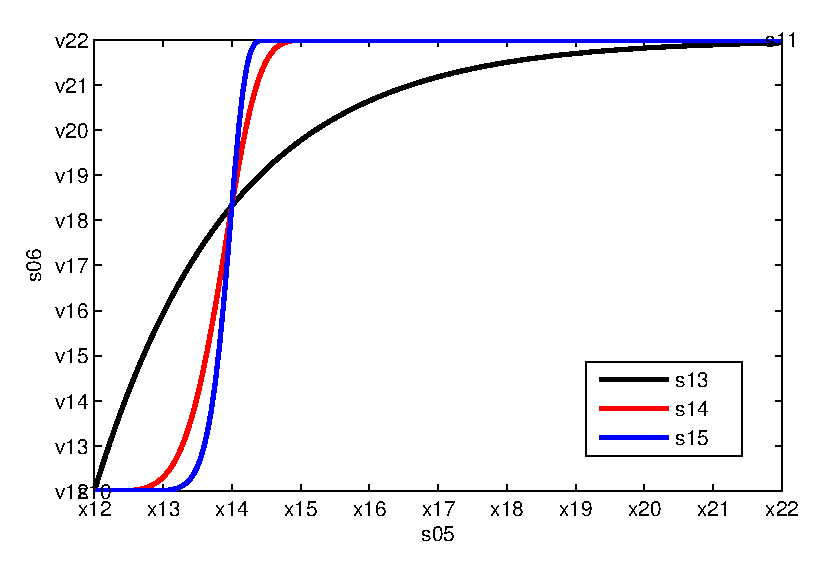
\includegraphics{./Images/Weibull.eps}}%
\end{psfrags}%
%
% End Weibull.tex
\end{document}
% See http://www.mathworks.de/matlabcentral/fileexchange/loadFile.do?objectId=4638
% for recent versions of laprint.m.
%
% created by:           LaPrint version 3.16 (13.9.2004)
% created on:           30-Dec-2013 09:44:00
% eps bounding box:     15 cm x 9.4415 cm
% comment:              
%
\begin{psfrags}%
\psfragscanon%
%
% text strings:
\psfrag{s05}[t][t]{\color[rgb]{0,0,0}\setlength{\tabcolsep}{0pt}\begin{tabular}{c}Applied Stress [Pa]\end{tabular}}%
\psfrag{s06}[b][b]{\color[rgb]{0,0,0}\setlength{\tabcolsep}{0pt}\begin{tabular}{c}Probability of Failure\end{tabular}}%
\psfrag{s10}[][]{\color[rgb]{0,0,0}\setlength{\tabcolsep}{0pt}\begin{tabular}{c} \end{tabular}}%
\psfrag{s11}[][]{\color[rgb]{0,0,0}\setlength{\tabcolsep}{0pt}\begin{tabular}{c} \end{tabular}}%
\psfrag{s12}[l][l]{\color[rgb]{0,0,0}m=10}%
\psfrag{s13}[l][l]{\color[rgb]{0,0,0}m=1}%
\psfrag{s14}[l][l]{\color[rgb]{0,0,0}m=5}%
\psfrag{s15}[l][l]{\color[rgb]{0,0,0}m=10}%
%
% xticklabels:
\psfrag{x01}[t][t]{0}%
\psfrag{x02}[t][t]{0.1}%
\psfrag{x03}[t][t]{0.2}%
\psfrag{x04}[t][t]{0.3}%
\psfrag{x05}[t][t]{0.4}%
\psfrag{x06}[t][t]{0.5}%
\psfrag{x07}[t][t]{0.6}%
\psfrag{x08}[t][t]{0.7}%
\psfrag{x09}[t][t]{0.8}%
\psfrag{x10}[t][t]{0.9}%
\psfrag{x11}[t][t]{1}%
\psfrag{x12}[t][t]{0}%
\psfrag{x13}[t][t]{1}%
\psfrag{x14}[t][t]{2}%
\psfrag{x15}[t][t]{3}%
\psfrag{x16}[t][t]{4}%
\psfrag{x17}[t][t]{5}%
\psfrag{x18}[t][t]{6}%
\psfrag{x19}[t][t]{7}%
\psfrag{x20}[t][t]{8}%
\psfrag{x21}[t][t]{9}%
\psfrag{x22}[t][t]{\shortstack{10\\$\times 10^{8}\ $}}%
%
% yticklabels:
\psfrag{v01}[r][r]{0}%
\psfrag{v02}[r][r]{0.1}%
\psfrag{v03}[r][r]{0.2}%
\psfrag{v04}[r][r]{0.3}%
\psfrag{v05}[r][r]{0.4}%
\psfrag{v06}[r][r]{0.5}%
\psfrag{v07}[r][r]{0.6}%
\psfrag{v08}[r][r]{0.7}%
\psfrag{v09}[r][r]{0.8}%
\psfrag{v10}[r][r]{0.9}%
\psfrag{v11}[r][r]{1}%
\psfrag{v12}[r][r]{0}%
\psfrag{v13}[r][r]{0.1}%
\psfrag{v14}[r][r]{0.2}%
\psfrag{v15}[r][r]{0.3}%
\psfrag{v16}[r][r]{0.4}%
\psfrag{v17}[r][r]{0.5}%
\psfrag{v18}[r][r]{0.6}%
\psfrag{v19}[r][r]{0.7}%
\psfrag{v20}[r][r]{0.8}%
\psfrag{v21}[r][r]{0.9}%
\psfrag{v22}[r][r]{1}%
%
% Figure:
\resizebox{9cm}{!}{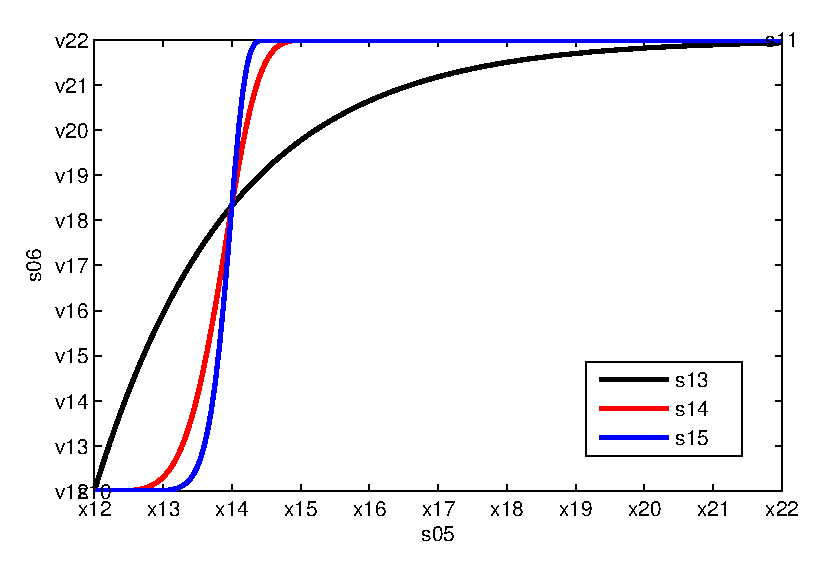
\includegraphics{./Images/Weibull.eps}}%
\end{psfrags}%
%
% End Weibull.tex
\end{document}
% See http://www.mathworks.de/matlabcentral/fileexchange/loadFile.do?objectId=4638
% for recent versions of laprint.m.
%
% created by:           LaPrint version 3.16 (13.9.2004)
% created on:           30-Dec-2013 09:44:00
% eps bounding box:     15 cm x 9.4415 cm
% comment:              
%
\begin{psfrags}%
\psfragscanon%
%
% text strings:
\psfrag{s05}[t][t]{\color[rgb]{0,0,0}\setlength{\tabcolsep}{0pt}\begin{tabular}{c}Applied Stress [Pa]\end{tabular}}%
\psfrag{s06}[b][b]{\color[rgb]{0,0,0}\setlength{\tabcolsep}{0pt}\begin{tabular}{c}Probability of Failure\end{tabular}}%
\psfrag{s10}[][]{\color[rgb]{0,0,0}\setlength{\tabcolsep}{0pt}\begin{tabular}{c} \end{tabular}}%
\psfrag{s11}[][]{\color[rgb]{0,0,0}\setlength{\tabcolsep}{0pt}\begin{tabular}{c} \end{tabular}}%
\psfrag{s12}[l][l]{\color[rgb]{0,0,0}m=10}%
\psfrag{s13}[l][l]{\color[rgb]{0,0,0}m=1}%
\psfrag{s14}[l][l]{\color[rgb]{0,0,0}m=5}%
\psfrag{s15}[l][l]{\color[rgb]{0,0,0}m=10}%
%
% xticklabels:
\psfrag{x01}[t][t]{0}%
\psfrag{x02}[t][t]{0.1}%
\psfrag{x03}[t][t]{0.2}%
\psfrag{x04}[t][t]{0.3}%
\psfrag{x05}[t][t]{0.4}%
\psfrag{x06}[t][t]{0.5}%
\psfrag{x07}[t][t]{0.6}%
\psfrag{x08}[t][t]{0.7}%
\psfrag{x09}[t][t]{0.8}%
\psfrag{x10}[t][t]{0.9}%
\psfrag{x11}[t][t]{1}%
\psfrag{x12}[t][t]{0}%
\psfrag{x13}[t][t]{1}%
\psfrag{x14}[t][t]{2}%
\psfrag{x15}[t][t]{3}%
\psfrag{x16}[t][t]{4}%
\psfrag{x17}[t][t]{5}%
\psfrag{x18}[t][t]{6}%
\psfrag{x19}[t][t]{7}%
\psfrag{x20}[t][t]{8}%
\psfrag{x21}[t][t]{9}%
\psfrag{x22}[t][t]{\shortstack{10\\$\times 10^{8}\ $}}%
%
% yticklabels:
\psfrag{v01}[r][r]{0}%
\psfrag{v02}[r][r]{0.1}%
\psfrag{v03}[r][r]{0.2}%
\psfrag{v04}[r][r]{0.3}%
\psfrag{v05}[r][r]{0.4}%
\psfrag{v06}[r][r]{0.5}%
\psfrag{v07}[r][r]{0.6}%
\psfrag{v08}[r][r]{0.7}%
\psfrag{v09}[r][r]{0.8}%
\psfrag{v10}[r][r]{0.9}%
\psfrag{v11}[r][r]{1}%
\psfrag{v12}[r][r]{0}%
\psfrag{v13}[r][r]{0.1}%
\psfrag{v14}[r][r]{0.2}%
\psfrag{v15}[r][r]{0.3}%
\psfrag{v16}[r][r]{0.4}%
\psfrag{v17}[r][r]{0.5}%
\psfrag{v18}[r][r]{0.6}%
\psfrag{v19}[r][r]{0.7}%
\psfrag{v20}[r][r]{0.8}%
\psfrag{v21}[r][r]{0.9}%
\psfrag{v22}[r][r]{1}%
%
% Figure:
\resizebox{9cm}{!}{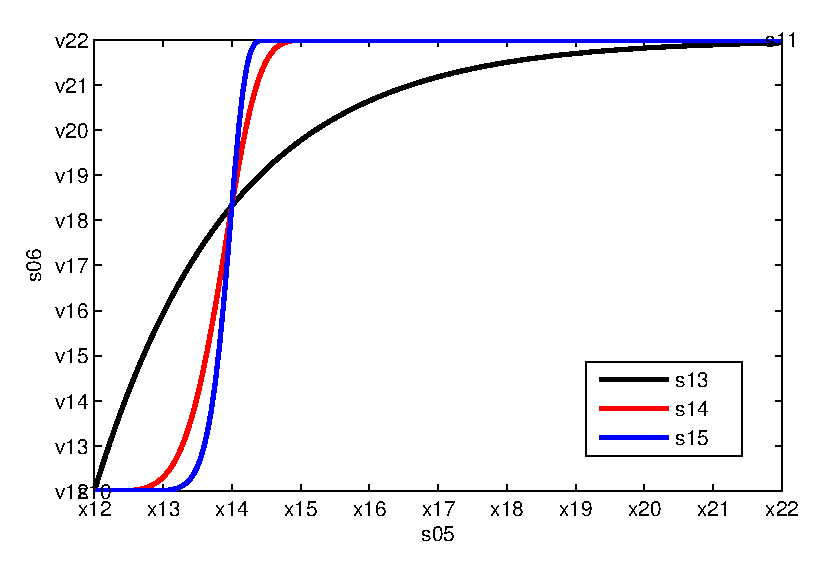
\includegraphics{./Images/Weibull.eps}}%
\end{psfrags}%
%
% End Weibull.tex

\caption{Plot of Weibull's assumpiton for various modulus m,  the values are: $\sigma_0=200 \mathrm{MPa}$, $k=1$.}
\label{fig:weibullsample}
\end{figure}

Weibull's strength theory of brittle materials is a pure statistical model. Weibull considered only the uni-axial stresses on his theory development and did not consider multiaxial stress state which is the case in reality. Weibull's  method has been the primary method until Batdorf's theory is published\cite{batdorf}. 
\subsection*{Batdorf's Theory}
In addition to the work of Weibull's that uses uniaxial stress state, Batdorf's theory considers also the multiaxial stress states in addition to Weibull's work\cite{batdorf}. Batdorf gives his main motivation on his publication saying :"Triaxial stress state requires close examination of the physical behaviour of the material".

In Batdorf's theory it is assumed that the fracture occurs when the effective stress $\sigma_e$ acting on the crack is equal to critical stress $\sigma_c$ which is defined as the remote tensile stress applied normal to the crack plane and caused the fracture. In this method, in addition to the stress state of Weibull's treatment, crack's orientations are also considered. A crack will have more probability of fracture under tensile stress and less probability of failure under stresses that are paralel to the crack plane. At conclusion, the probability of fracture of a crack is given by the equation
\begin{align}
S=e^{-\int\int\int dV d \Omega d\sigma_c H\left(\sigma_e, \sigma_c\right)\cfrac{d N}{d \sigma_c}}
\label{equ:batdorf}
\end{align}
where $\Omega$ is the range of angle of cracks where $\sigma>\sigma_c$ and
\begin{align}
H\left(\sigma_e,\sigma_c\right)&=1\quad \text{when}\quad \sigma_e>\sigma_c\\
&=0\quad \text{when}\quad \sigma_e<\sigma_c
\end{align}
The effective stress causing the fracture is a function of both the component of the stress normal to the crack plane, $\sigma_n$, and the shear stress $\tau$ parallel to the crack plane. The physical background of Batdorf's probability of failure in \cref{equ:batdorf} is more readily apparent while Weibull's method is computationally more convinient.

\section{Experiments}
Experiments are one of the core part of the statistical modeling of ceramic materials. There are kinds of experiments to simulate in situ stress conditions then express the possibility of failure under that stress state. The experiments are used to fit statistical methods to model the specimens. The usual way of the experimental fit processes follow the steps below
\begin{itemize}
\item{ Collect $\sigma$ where specimens fails}
\item{ Determine the $m$ and $k$ for the Weibull parameters}
\end{itemize}
A summary of the type of experiments are given in \cref{fig:experiments}.\newline 

\begin{figure}[ht!]
\centering
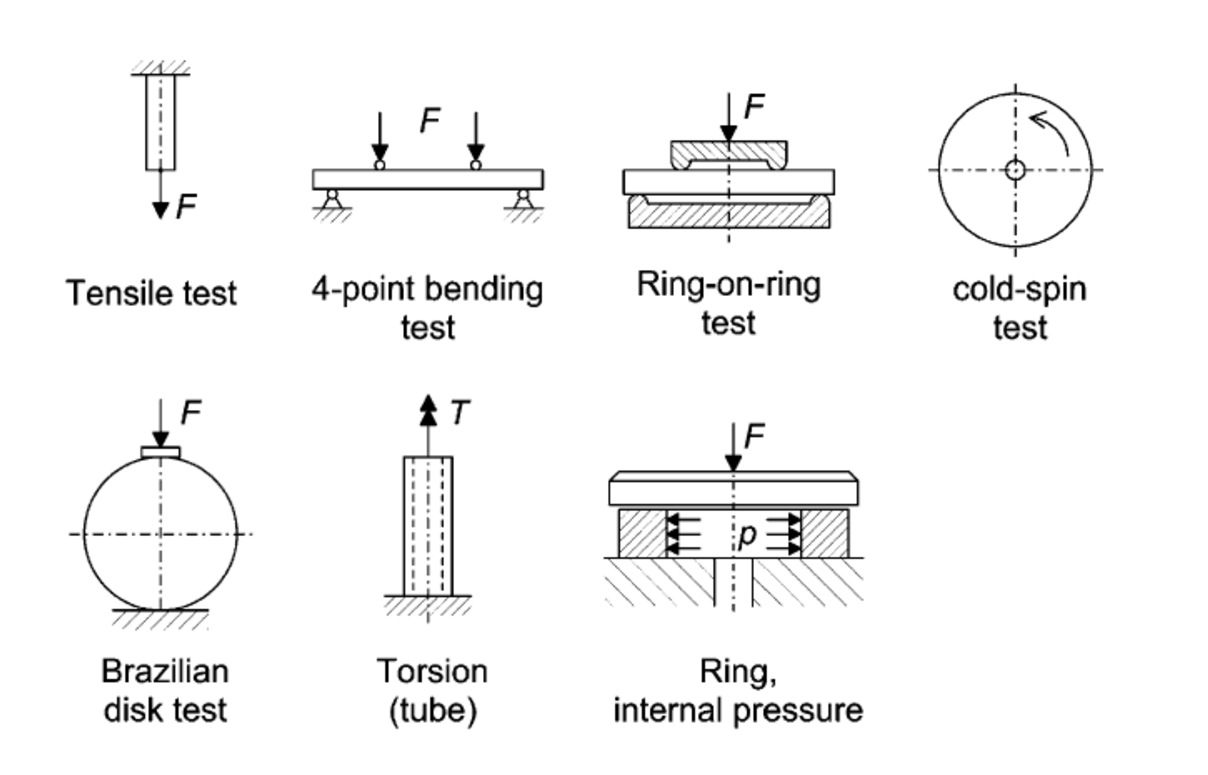
\includegraphics[width=0.7\linewidth]{./Figures/experiments}
\caption{Experiments that are done for the fitting of the statistical ceramic materials\cite{Sheunemann}.}
\label{fig:experiments}
\end{figure}
 

The experiments of statistical fracture of ceramic materials can be both in the form of laboratory experiments or numerical simulations. 
Since, except the case in which creating the computer model of material requires more effort than the real experiments, 
computer simulations are always preferred. At this point, it is meaningful to introduce computer analysis tools. 
Currently, the only numerical tool for the fracture analysis of ceramics is the CARES(ceramic analysis and 
reliability evaluation of structures)\cite{nemeth} that is first developed by NASA and now hold by a commercial company.

CARES includes a number of fracture theories to predict material response due to multiaxial stresses. They include Weibull model, Normal stress averaging, Principle of independent action and Batdorf's model. From these models Batdorf's model is advised. The simulations within CARES is done with third party finite element programs MSC/NASTRAN and ANSYS with using the elastostatic analysis output. Although CARES seems very handy and complete tool for the analysis of ceramic materials, it is currently under development.
\section*{Conclusion}
In this paper, core methods of the statistical methods of fast fracture of ceramics are reviewed where brittleness makes use of statistical approach is a must. Also, the reasons for requirement of the statistical methods and variable types of them is mentioned. Although, there are numbers of different models, they are all based on the Weibull's work and they varies with the including and excluding the physics of fracture.


\bibliography{bibliography}
\bibliographystyle{ieeetr}
\end{document}
